
%% bare_jrnl_compsoc.tex
%% V1.4a
%% 2014/09/17
%% by Michael Shell
%% See:
%% http://www.michaelshell.org/
%% for current contact information.
%%
%% This is a skeleton file demonstrating the use of IEEEtran.cls
%% (requires IEEEtran.cls version 1.8a or later) with an IEEE
%% Computer Society journal paper.
%%
%% Support sites:
%% http://www.michaelshell.org/tex/ieeetran/
%% http://www.ctan.org/tex-archive/macros/latex/contrib/IEEEtran/
%% and
%% http://www.ieee.org/

%%*************************************************************************
%% Legal Notice:
%% This code is offered as-is without any warranty either expressed or
%% implied; without even the implied warranty of MERCHANTABILITY or
%% FITNESS FOR A PARTICULAR PURPOSE! 
%% User assumes all risk.
%% In no event shall IEEE or any contributor to this code be liable for
%% any damages or losses, including, but not limited to, incidental,
%% consequential, or any other damages, resulting from the use or misuse
%% of any information contained here.
%%
%% All comments are the opinions of their respective authors and are not
%% necessarily endorsed by the IEEE.
%%
%% This work is distributed under the LaTeX Project Public License (LPPL)
%% ( http://www.latex-project.org/ ) version 1.3, and may be freely used,
%% distributed and modified. A copy of the LPPL, version 1.3, is included
%% in the base LaTeX documentation of all distributions of LaTeX released
%% 2003/12/01 or later.
%% Retain all contribution notices and credits.
%% ** Modified files should be clearly indicated as such, including  **
%% ** renaming them and changing author support contact information. **
%%
%% File list of work: IEEEtran.cls, IEEEtran_HOWTO.pdf, bare_adv.tex,
%%                    bare_conf.tex, bare_jrnl.tex, bare_conf_compsoc.tex,
%%                    bare_jrnl_compsoc.tex, bare_jrnl_transmag.tex
%%*************************************************************************


% *** Authors should verify (and, if needed, correct) their LaTeX system  ***
% *** with the testflow diagnostic prior to trusting their LaTeX platform ***
% *** with production work. IEEE's font choices and paper sizes can       ***
% *** trigger bugs that do not appear when using other class files.       ***                          ***
% The testflow support page is at:
% http://www.michaelshell.org/tex/testflow/


\documentclass[10pt,conference,onecolumn,compsoc]{IEEEtran}


\usepackage{hyperref}
\usepackage{enumitem}
\setlist[itemize]{leftmargin=3 cm}
\setlist[enumerate]{leftmargin=3cm}



% *** CITATION PACKAGES ***
%
\ifCLASSOPTIONcompsoc
  % IEEE Computer Society needs nocompress option
  % requires cite.sty v4.0 or later (November 2003)
  \usepackage[nocompress]{cite}
\else
  % normal IEEE
  \usepackage{cite}
\fi
% cite.sty was written by Donald Arseneau
% V1.6 and later of IEEEtran pre-defines the format of the cite.sty package
% \cite{} output to follow that of IEEE. Loading the cite package will
% result in citation numbers being automatically sorted and properly
% "compressed/ranged". e.g., [1], [9], [2], [7], [5], [6] without using
% cite.sty will become [1], [2], [5]--[7], [9] using cite.sty. cite.sty's
% \cite will automatically add leading space, if needed. Use cite.sty's
% noadjust option (cite.sty V3.8 and later) if you want to turn this off
% such as if a citation ever needs to be enclosed in parenthesis.
% cite.sty is already installed on most LaTeX systems. Be sure and use
% version 5.0 (2009-03-20) and later if using hyperref.sty.
% The latest version can be obtained at:
% http://www.ctan.org/tex-archive/macros/latex/contrib/cite/
% The documentation is contained in the cite.sty file itself.



% *** GRAPHICS RELATED PACKAGES ***
%
\ifCLASSINFOpdf
   \usepackage[pdftex]{graphicx}
 
\else
 
\fi
% graphicx was written by David Carlisle and Sebastian Rahtz. It is
% required if you want graphics, photos, etc. graphicx.sty is already
% installed on most LaTeX systems. The latest version and documentation
% can be obtained at: 
% http://www.ctan.org/tex-archive/macros/latex/required/graphics/
% Another good source of documentation is "Using Imported Graphics in
% LaTeX2e" by Keith Reckdahl which can be found at:
% http://www.ctan.org/tex-archive/info/epslatex/
%
% latex, and pdflatex in dvi mode, support graphics in encapsulated
% postscript (.eps) format. pdflatex in pdf mode supports graphics
% in .pdf, .jpeg, .png and .mps (metapost) formats. Users should ensure
% that all non-photo figures use a vector format (.eps, .pdf, .mps) and
% not a bitmapped formats (.jpeg, .png). IEEE frowns on bitmapped formats
% which can result in "jaggedy"/blurry rendering of lines and letters as
% well as large increases in file sizes.
%
% You can find documentation about the pdfTeX application at:
% http://www.tug.org/applications/pdftex









% *** PDF, URL AND HYPERLINK PACKAGES ***
%
\usepackage{url}
% url.sty was written by Donald Arseneau. It provides better support for
% handling and breaking URLs. url.sty is already installed on most LaTeX
% systems. The latest version and documentation can be obtained at:
% http://www.ctan.org/tex-archive/macros/latex/contrib/url/
% Basically, \url{my_url_here}.



\begin{document}

% found this here: https://stackoverflow.com/questions/1211888/is-there-any-way-i-can-define-a-variable-in-latex
\newcommand\projname{Vapor}

\title{\projname, A PC Game Library Manager}
%
%

% received ..."  text while in non-compsoc journals this is reversed. Sigh.

\author{Steven Gray and Andy Lum% <-this % stops a space
}

\IEEEtitleabstractindextext{%
\begin{abstract}
In the modern era of PC gaming, its too easy to lose track of games. Many of the biggest games are spread across multiple launchers, while a lot of smaller games find themselves disconnected from all of them. That's where Vapor comes in. \projname{} is a minamalist game library manager to help gamers keep track of all of their games across various launchers. This proposal document is the bulk of what we've done so far.
\end{abstract}

}


% make the title area
\maketitle



\IEEEdisplaynontitleabstractindextext

\IEEEpeerreviewmaketitle



\section{Introduction}

Increasing popularity of PC gaming has lead to a unique situation where many of the biggest developers want to create their own storefronts and game libraries to maximize the amount of profit they make on a game sale. This becomes a hassle for gamers who simply want to play their games without having to sift through multiple different programs to find where their game is hiding.

\subsection{Background}
This issue is further exacerbated by storefronts without their own launchers, or programs managed by storefronts/developers to sell their games, leading to a collection of stray programs on your computer that you download to play one or two games.

Vapor exists to solve this problem. Vapor is a video game library manager, a program that allows a user to manage their library of video games.

\subsection{Impacts}
At the very least, our goal is to make game management easier and more flexible for the user. We want to create an environment where someone can avoid wasting time sifting through folders or launchers just to find what game they want to play, or avoid wasting money buying games they already own because they simply can't find what they're looking for.

\subsection{Challenges}
The immediate challenges this project brings up include determining what the name of a particular game is, finding the launcher that the game is associated with, and figuring out how to work with online databases.

\section{Scope}
The initial goal for this project is to create a functional interface that allows for a user to have all of their games accessible and playable through a single library manager. This would include:

\begin{itemize}
\item A main menu with all of their games available and playable.
\item An options menu that would allow a user to add new games or treat certain folders as library folders (alongside an automatically created library folder handled by the program itself).
\item The ability to remove a game or library folder from the library manager or delete them altogether
\item The ability to refresh the library at any time, to find newly added games or remove recently removed ones.
\item The ability to open the location where a game is stored
\end{itemize}

A few possible stretch goals could be:

\begin{itemize}
\item Offline Mode, a way to use the launcher without needing to connect to any databases (with possibly limited functionality)
\item Icons that allow for a user to discern where the games are from, such as Steam, Battle.net, or a user defined Library folder.
\item A store page that allows a user to search/browse popular storefronts like Steam, GOG, and Humble.
\item Allow the user to create and manage groups of games
\end{itemize}

\subsection{Requirements}
As part of fleshing out the scope of your requirements, you'll also need to keep in mind both your functional and non-functional requirements.  These should be listed, and explained in detail as necessary.  Use this area to explain how you gathered these requirements.

\subsubsection{Functional}

\begin{itemize}
\item User needs to have a locally stored list of games on the computer - including their locations and any necessary assets such as cover art or icons
\item User needs to have cover art and icons for each game
\item User needs to be able to launch games from the program
\end{itemize}

\subsubsection{Non-Functional}

\begin{itemize}
\item Game information has to be saved somewhere convenient to reference whether online or offline 
\end{itemize}

%
%\subsubsection{Functional}
%\begin{itemize}
%\item User needs to have a private shopping cart -- this cannot be shared between users, and needs to maintain state across subsequent visits to the site
%\item Users need to have website accounts -- this will help track recent purchases, keep shopping cart records, etc.
%\item You'll need more than 2 of these...
%\end{itemize}
%
%\subsubsection{Non-Functional}
%\begin{itemize}
%\item Security -- user credentials must be encrypted on disk, users should be able to reset their passwords if forgotten
%\item you'll typically have fewer non-functional than functional requirements
%\end{itemize}
%
\subsection{Use Cases}
%This subsection is arguably part of how you define your project scope (why it is in the Scope section...).  In a traditional Waterfall approach, as part of your requirements gathering phase (what does the product actually \emph{need} to do?), you will typically sit down with a user to develop use cases.
%
%You should have a table listing all use cases discussed in the document, the ID is just the order it is listed in, the name should be indicative of what should happen, the primary actor is typically most important in an application where you may have different levels of users (think admin vs normal user), complexity is a best-guess on your part as to how hard it should be.  A lower number in priority indicates that it needs to happen sooner rather than later.  A sample table, or Use Case Index can be seen in Table \ref{tab:useCaseIndex}.
%
%
%
%
%\begin{table}
%\centering
%\begin{tabular}{|c|c|c|c|c|}
%\hline
%Use Case ID & Use Case Name & Primary Actor & Complexity & Priority \\
%\hline \hline
%1 & Add item to cart & Shopper & Med & 1\\
%\hline
%2 & Checkout & Shopper & Med & 1\\
%\hline

%\end{tabular}
%\caption{Sample use case table}
%\label{tab:useCaseIndex}
%\end{table}


\begin{itemize}
\item[Use Case Number:] 1
\item[Use Case Name:] Add a game to list
\item[Description:] A user wants to add a single game to their list. They open up a settings drop-down and click on an "Add Game To Vapor" button. This will then allow the user to select the file they want to add and subsequently add it to the program
\end{itemize}
%
%You will then go on to (minimally) discuss a basic flow for the process:
%
\begin{enumerate}
\item User opens up the settings menu.
\item User left-clicks on "Add Game To Vapor" button.
\item User searches for and selects their game.
\item The program finds everything needed and adds it to the user's list
\item[Termination Outcome:] The game the user selected is added to their list.
\end{enumerate}
%
%You may need to also add in any alternative flows:
%
Alternative: Game exists in list
\begin{enumerate}
\item User opens up the settings menu.
\item User left-clicks on "Add Game To Vapor" button.
\item User searches for and selects their game.
\item [Termination Outcome:] A message pops up telling the user that the game is already available in their list, and the screen returns to the main list page.
\end{enumerate}
%
%You will often also need to include pictures or diagrams.  It is quite common to see use-case diagrams in such write-ups.  To properly reference an image, you will need to use the \texttt{figure} environment and will need to reference it in your text (via the \texttt{ref} command) (see Figure \ref{cat1}).  NOTE: this is not a use case diagram, but a kitten.
%
%After fully describing a use case, it is time to move on to the next use case:
%
\begin{itemize}
\item[Use Case Number:] 2
\item[Use Case Name:] Add a folder of games to list
\item[Description:] A user wants to add a folder of games to the list. They open up a settings drop-down and click on an "Add Library Folder To Vapor" button. This will then allow the user to select the file they want to a dd and subsequently add it to the program.
\end{itemize}

\begin{enumerate}
\item User opens up the settings menu.
\item User left-clicks on "Add Library Folder To Vapor"
\item User searches for and selects the folder they want to add.
\item The program searches through the folder for any games it can find and adds them to the list.
\item[Termination Outcome:] The folder is added to the program, and the games inside of it are added to the list.
\end{enumerate}

Alternative: The folder has already been added
\begin{enumerate}
\item User opens up the settings menu.
\item User left-clicks on "Add Library Folder To Vapor"
\item User searches for and selects the folder they want to add.
\item[Termination Outcome:] A message pops up saying the folder already exists in the program and returns to the list screen.
\end{enumerate}

\begin{itemize}
\item[Use Case Number:] 3
\item[Use Case Name:] Launch a game from Vapor
\item[Description:] A user wants to play a game. They left click on the game they want to play from their list, and then left click a "Play" button.
\end{itemize}

\begin{enumerate}
\item User left-clicks on the game they want to launch from their list.
\item User navigates over to a large "Play" button
\item[Termination Outcome:] The game is run.
\end{enumerate}

%
%You will then need to continue to flesh out all use cases you have identified for your project.
%
%\begin{figure}[ht!]
%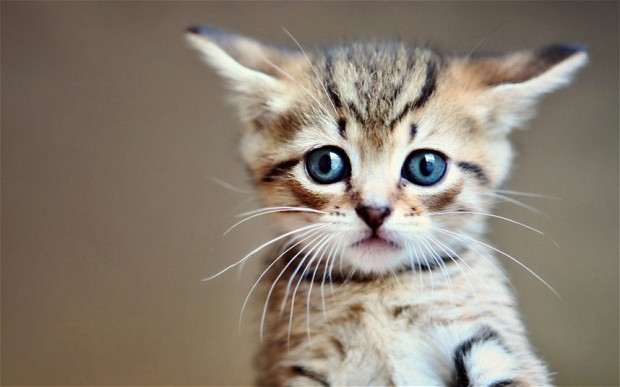
\includegraphics[height=250px, width=350px]{cat1.jpg}
%\caption{First picture, this is a kitten, not a use case diagram}
%\label{cat1}
%\end{figure}
%
\subsection{Interface Mockups}
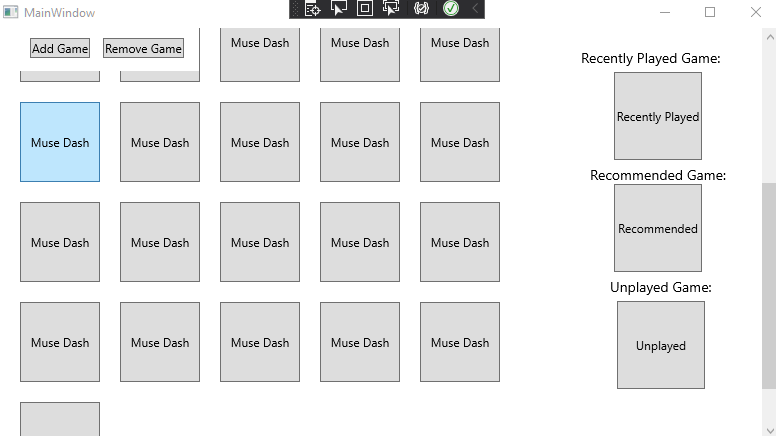
\includegraphics[width=6in]{mainwindow_final.png}

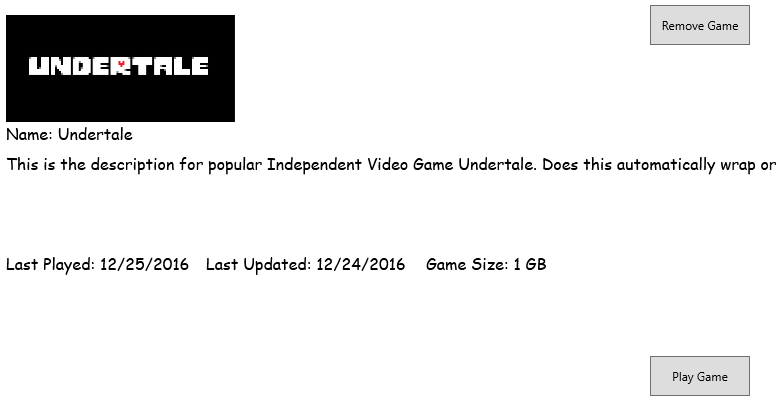
\includegraphics[width=6in]{gamewindow.png}
%\section{Project Timeline}
%Go back to your notes and look up a typical project development life cycle for the Waterfall approach.  How will you follow this life cycle over the remainder of this semester?  This will usually involve a chart showing your proposed timeline, with specific milestones plotted out.  Make sure you have deliverable dates from the course schedule listed, with a plan to meet them (NOTE: these are generally optimistic deadlines).
%
\section{Project Structure}
At first, this will be a little empty (it will need to be filled in by the time you turn in your final report).  This is your chance to discuss all of your design decisions (consider this the README's big brother).
%
%\subsection{UML Outline}
%Show the full structure of your program.  Make sure to keep on updating this section as your project evolves (you often start out with one plan, but end up modifying things as you move along).  As a note, while Dia fails miserably at generating pdfs (probably my fault), I have had much success with png files.  Make sure to wrap your images in a \texttt{figure} environment, and to reference with the \texttt{ref} command.  For example, see Figure \ref{cat2}.
%
%\begin{figure}[ht!]
%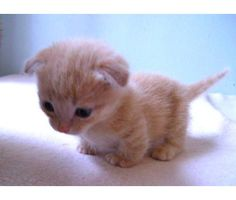
\includegraphics[scale=1.5]{cat2.jpg}
%\caption{Your figures should be in the \emph{figure} environment, and have captions.  Should also be of diagrams pertaining to your project, not random internet kittens}
%\label{cat2}
%\end{figure}
%
%
\subsection{Design Patterns Used}
Factory pattern and Observer pattern.
%Make sure to actually use at least 2 design patterns from this class.  This is not normally part of such documentation, but largely just specific to this class -- I want to see you use the patterns!
%
%
%\section{Results}
%This section will start out a little vague, but it should grow as your project evolves.  With each deliverable you hand in, give me a final summary of where your project stands.  By the end, this should be a reflective section discussing how many of your original goals you managed to attain/how many desired use cases you implemented/how many extra features you added.
%
\subsection{Future Work}
Once this class is over, I'll delete the program from my computer and likely eventually forget about it.
%Where are you going next with your project?
%For early deliverables, what are your next steps?  (HINT: you will typically want to look back at your timeline and evaluate: did you meet your expected goals?  Are you ahead of schedule?  Did you decide to shift gears and implement a new feature?)
%By the end, what do you plan on doing with this project?  Will you try to sell it?  Set it on fire?  Link to it on your resume and forget it exists?
%
%
%
%\begin{IEEEbiography}{Michael Shell}
%Biography text here.
%\end{IEEEbiography}
%
%% if you will not have a photo at all:
%\begin{IEEEbiographynophoto}{John Doe}
%Biography text here.
%\end{IEEEbiographynophoto}
%
%% insert where needed to balance the two columns on the last page with
%% biographies
%%\newpage
%
%\begin{IEEEbiographynophoto}{Jane Doe}
%Biography text here.
%\end{IEEEbiographynophoto}
%
%



% that's all folks
\end{document}


